\documentclass{article}
\usepackage{spconf,amsmath,graphicx,hyperref}
\usepackage{amsmath}
\usepackage[flushleft]{threeparttable}
\usepackage{cite}
\usepackage{booktabs, multirow}
\usepackage{enumitem} %缩进itemize
\usepackage{amssymb}

\usepackage[table]{xcolor}
\usepackage{pgf}

\definecolor{heatblue}{RGB}{65,115,200}
\definecolor{heatred}{RGB}{205,92,92}

\newcommand{\heatpos}[1]{%
  \pgfmathtruncatemacro{\shadevalue}
    {min(54,14+40*sqrt((#1)/10))}%
  \edef\heatcolor{heatblue!\shadevalue}%
  \expandafter\cellcolor\expandafter{\heatcolor}%
  $+$#1%
}

\newcommand{\heatneg}[1]{%
  \pgfmathtruncatemacro{\shadevalue}
    {min(54,14+40*sqrt((#1)/10))}%
  \edef\heatcolor{heatred!\shadevalue}%
  \expandafter\cellcolor\expandafter{\heatcolor}%
  $-$#1%
}

\newcommand{\heatposbest}[1]{%
  \pgfmathtruncatemacro{\shadevalue}
    {min(54,14+40*sqrt((#1)/10))}%
  \edef\heatcolor{heatblue!\shadevalue}%
  \expandafter\cellcolor\expandafter{\heatcolor}%
  $\mathbf{+}$\textbf{#1}%
}

\newcommand{\heatnegbest}[1]{%
  \pgfmathtruncatemacro{\shadevalue}
    {min(54,14+40*sqrt((#1)/10))}%
  \edef\heatcolor{heatred!\shadevalue}%
  \expandafter\cellcolor\expandafter{\heatcolor}%
  $\mathbf{-}$\textbf{#1}%
}

% \usepackage{lilyglyphs} % dynamic symbols
% \usepackage{tikz}
% \usetikzlibrary{arrows.meta,positioning,fit,calc}
% \tikzset{
%   block/.style={draw, rounded corners, very thick, align=center, inner sep=3pt, minimum height=8mm, fill=white},
%   tinyblock/.style={draw, rounded corners, thick, inner sep=2pt, minimum height=4mm, fill=white},
%   arrow/.style={-Latex, very thick}
% }

\title{CASM: A Context-Aware Semi-Markov Alternative to DBN Post-Processor for Beat Tracking}

\name{Zhanhong He$^{1}$, Hanyu Meng$^{2}$, Yaolong Ju$^{3}$}
\address{
    $^{1}$The University of Western Australia, Perth, Australia\\
    $^{2}$The University of New South Wales, Sydney, Australia\\
    $^{3}$Great Bay University, Guangdong, China
}

\begin{document}
\ninept
\maketitle

\begin{abstract}
The last stage of beat tracking must turn dense neural activations into a discrete, musically coherent event sequence. Direct peak picking preserves local evidence but can produce fragmented or duplicated beat events, whereas dynamic Bayesian networks (DBNs), the dominant post-processing approach, suppress such errors through explicit human-specified global assumptions (e.g., tempo, meter). However, these assumptions often become unreliable across diverse and complex music. We address this with CASM, a model-agnostic, context-aware semi-Markov decoder that exploits local structure in beat activations. CASM estimates local periodicity and ambiguity from the activations, then commits strongly when the cues are clear and relaxes toward the neural output when they are ambiguous, with built-in safeguards keeping this behavior stable and predictable. With a single calibrated configuration, CASM improves F1, CMLt, and AMLt across BeatThis, MSCNN, and TCN models on GTZAN, and delivers state-of-the-art performance on SMC. Further analysis shows that CASM is less sensitive than DBNs to the choice of calibration data.\footnote{Code and demo are available at \url{https://zhanh-he.github.io/casm-icassp2026-plot}.}
\end{abstract}

\begin{keywords}
beat tracking, downbeat, content-aware, semi-Markov decoding, post-processing, local periodicity
\end{keywords}


\section{Introduction}
\label{sec:intro}
Despite recent attempts to remove post-processing from neural beat tracking \cite{chen2022postprocessingfree,foscarin2024beat}, many modern systems still rely on structured decoders such as dynamic Bayesian networks (DBNs) to obtain musically coherent beat estimates \cite{krebs2015dbn}. Even with increasingly accurate neural activations, framewise predictions do not directly guarantee a coherent event sequence: direct peak picking can produce duplicated or missing beats, metrical-level switches, or downbeats that disagree with the beat grid. Post-processing therefore remains useful for converting local activation evidence into a temporally consistent sequence. The central difficulty is how strongly this temporal structure should be imposed: weak decoding follows the network closely but can sacrifice continuity, whereas strong decoding can override correct evidence under expressive or unusual timing.

DBNs address this problem by decoding a path through tempo, phase, and meter states under transition assumptions specified before the track is observed \cite{krebs2015dbn,bock2016joint}. This is effective when assumptions such as the BPM range, allowed meters, and tempo-transition law match the input, but corpus-specific retuning can become necessary for music outside these global assumptions \cite{ahn2026smcblindspot}. PLPDP provides a more local alternative: it estimates a time-varying inter-beat interval and confidence from predominant local pulse (PLP), and uses them to adapt the temporal constraint during dynamic programming \cite{chiu2023localperiodicity}. This establishes an important principle for activation decoding: the temporal prior can depend on the local evidence itself. However, the strongest local period need not be decisive. Half- and double-tempo hypotheses can receive similar support, in which case strongly enforcing either interpretation may be undesirable.

We introduce CASM, a context-aware semi-Markov decoder that makes this distinction explicit. CASM constructs a sparse path over activation-supported peaks and estimates both local periodicity and its ambiguity. These estimates control the target, strength, and tolerance of the segment-duration preference: when the periodic evidence is clear, CASM commits strongly to local regularity; when competing periods are similarly plausible, it weakens that preference and lets the neural activations dominate. Fig.~\ref{fig:casm-examples} illustrates both cases. On the left, clear local periodicity allows CASM to recover weak, activation-supported beats that Direct misses; on the right, competing periodicity hypotheses make CASM defer to the Direct path. A beat-count safeguard and beat-synchronous meter decoder further keep the procedure deterministic and predictable. CASM is a model-agnostic plug-in that requires neither backbone retraining nor per-track BPM or meter tuning, and we provide it with a single calibrated configuration for direct use (also showing lower sensitivity than DBNs to the choice of calibration data).

\begin{figure}[htbp]
\centering
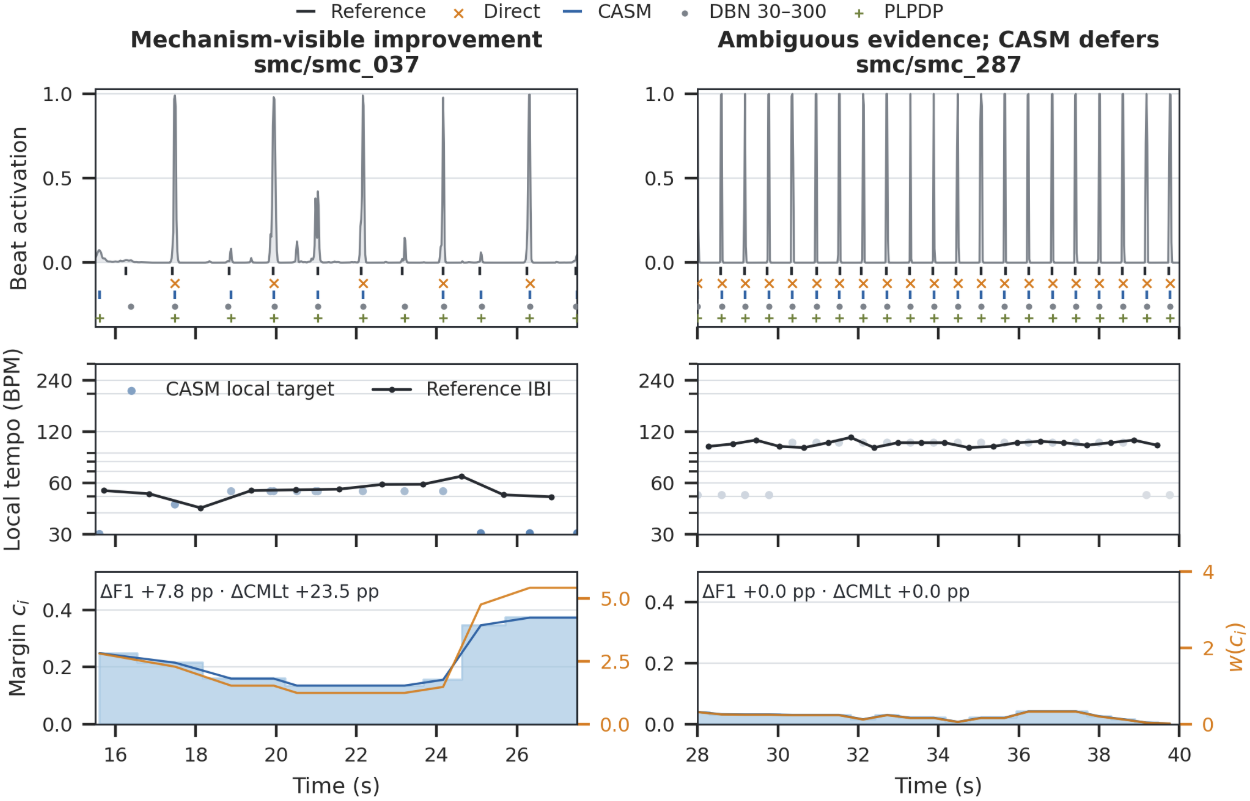
\includegraphics[width=\columnwidth]{figures/p0.jpg}
\caption{Illustrative CASM behaviour on held-out Beat This activations from SMC. Clear local periodicity recovers weak activation-supported beats (left), whereas ambiguous competing periods make CASM defer to Direct (right). Reference IBI is shown only for interpretation.}
\label{fig:casm-examples}
\end{figure}


\section{Related Work}
\label{sec:related}

\subsection{Structured post-processing}

Dynamic programming has long balanced onset evidence against inter-beat
regularity \cite{ellis2007beattracking}. Bayesian beat-position models used a
dominant beat interval \cite{korzeniowski2014crf}, while learned CRFs were later
extended from beats to downbeats, long-range section consistency, and
genre-specific microtiming \cite{fillon2015crf,durand2016crfdownbeat,
fuentes2019skipchain,fuentes2019microtiming}. Resonating comb filters estimate a
dominant periodicity before event alignment \cite{bock2015combfilter}, and DBNs
enumerate tempo--phase--meter states and decode their most likely trajectory
\cite{krebs2015dbn,bock2016joint}. These methods differ in state representation
and optimization, but they share a useful principle: noisy framewise evidence
should be interpreted as a sequence rather than thresholded independently.

\subsection{From PLPDP to ambiguity-aware local constraints}

PLPDP is CASM's direct methodological predecessor
\cite{chiu2023localperiodicity}. Its central diagnosis was that a fixed global
tempo penalty, including the empirically chosen transition law of common HMM
trackers, can be too rigid for expressive timing. PLPDP extracts a time-varying
inter-beat interval and a confidence curve from PLP, then replaces the global
target and weight of dense-frame dynamic programming with those local
quantities. Its real-time continuation improves controllability
\cite{meier2024realtime}, and dPLP makes local-pulse estimation differentiable
\cite{chiu2025dplp}.

% CASM advances this line of work rather than treating PLPDP as an unrelated
% baseline. PLPDP asks, ``What is the current local pulse, and how strong is its
% PLP peak?'' CASM additionally asks, ``How decisively does that pulse beat the
% next plausible explanation?'' It measures a top-versus-runner-up period margin
% around each retained activation maximum, combines the two endpoint contexts,
% and uses the result to change both the strength and the tolerance of a complete
% event-to-event duration cost. The path is sparse and remains anchored to
% observed maxima, whereas PLPDP can evaluate every frame. This extension is
% designed for half/double-tempo competition: when no period wins clearly, the
% decoder should not enforce any of them confidently.

Reliability-informed tracking previously established the broader principle
that temporal commitment should depend on evidence quality
\cite{degara2012reliability}. CASM's margin is a local, deterministic separation
score rather than predicted track-level accuracy. It also differs from the
causal one-dimensional semi-Markov state space of \cite{heydari2022semimarkov},
which maintains a framewise posterior and adapts a jump-back distribution
online. CASM is an offline maximum-score path over candidate-to-candidate
segments. Nor is it a semi-CRF: its potentials are hand-specified, unnormalized,
and not learned \cite{sarawagi2004semimarkov}.

\subsection{Alternatives beyond plug-in decoding}

Particle filters maintain online tempo hypotheses \cite{hainsworth2004particle},
and BeatNet/BeatNet+ extend this branch to joint real-time rhythm analysis
\cite{heydari2021beatnet,heydari2024beatnetplus}. Another line adapts a tracker
with user annotations \cite{pinto2021userdriven,maia2022adapting,
pinto2023bridging,maia2024selective,pinto2026challenging}. More recent systems
remove or redesign post-processing: masked diffusion iteratively refines
coherent sequences \cite{foscarin2026masked}, BeatFCOS predicts intervals as
objects with Soft-NMS \cite{ahn2025beatfcos}, and other work reformulates the
prediction target \cite{bolt2026reformulated}. These approaches change the
predictor or import additional supervision. CASM instead addresses the
deployment setting in which only the activation output of a frozen tracker is
available.

\section{Methodology}
\label{sec:method}

\subsection{Overview and PLPDP lineage}
\label{sec:casm}
Let a frozen tracker produce beat and downbeat logits $z_t^{\mathrm b}$ and
$z_t^{\mathrm d}$ at frame rate $F$. Like PLPDP, CASM derives a local period
and a measure of its support from the current beat activation. CASM then makes
two changes. First, it decodes only a sparse set of activation maxima rather
than every frame. Second, its support measure is the separation between the
best and competing periods, and it controls both how strongly and how narrowly
the chosen period is enforced. The global coefficients define one frozen
evidence-to-constraint rule; the input determines the operating point of that
rule at every candidate segment.

\subsection{Candidate-event segments}
Set $a_t=\operatorname{sigmoid}(z_t^{\mathrm b})$ and retain its local maxima
above threshold $\theta_{\mathrm c}$ as
$\mathcal C=\{t_1,\ldots,t_N\}$. An edge $(i,j)$ spans the complete elapsed
time $\Delta_{ij}=(t_j-t_i)/F$ and is allowed only within the 30--300 BPM
support. With $e_i$ denoting clipped activation evidence, CASM selects a path
$\pi=(i_1,\ldots,i_K)$ that maximizes
\begin{equation}
\mathcal S(\pi)=\sum_{k=1}^{K}e_{i_k}
-\sum_{k=2}^{K}D_{i_{k-1},i_k},
\label{eq:casm-objective}
\end{equation}
where $D_{ij}$ is the segment-duration cost below. This is the precise sense in
which CASM is semi-Markov: one transition consumes a variable-length
candidate-to-candidate segment and scores its duration as a whole. It is not a
generative hidden semi-Markov model, and the segment potentials are not learned.

\subsection{Local period and ambiguity}

At each candidate $i$, normalized autocorrelation scores the admissible integer
lags $\ell$ in a centred local window $\mathcal W_i$:
\begin{equation}
q_i(\ell)=
\frac{\left\langle a_u a_{u-\ell}\right\rangle_{u\in\mathcal W_i}}
{\sqrt{\left\langle a_u^2\right\rangle_{u\in\mathcal W_i}
       \left\langle a_{u-\ell}^2\right\rangle_{u\in\mathcal W_i}
       +\epsilon_q}}
\left(\frac{\ell_{\min}}{\ell}\right)^{\beta},
\label{eq:casm-local-period}
\end{equation}
with zero padding outside the signal and a mild fast-tempo prior in the final
factor. The winning lag gives $\ell_i^\star=\arg\max_\ell q_i(\ell)$ and local
period $\tau_i=\ell_i^\star/F$. We then compare it with the best lag outside a
$\pm2$-frame neighbourhood:
\begin{equation}
c_i=\operatorname{clip}_{[0,1]}\!\left(
\frac{q_i(\ell_i^\star)-
\max_{\ell:\,|\ell-\ell_i^\star|>2}q_i(\ell)}
{|q_i(\ell_i^\star)|+\epsilon_c}\right).
\label{eq:casm-reliability}
\end{equation}
Here $c_i$ is a period-separation margin, not a calibrated probability of being
correct. A large value means that one local period clearly wins; a small value
means that nearby or half/double-time explanations remain competitive. Both
$\tau_i$ and $c_i$ are median-filtered over five consecutive candidates.

\subsection{Ambiguity-conditioned segment cost}

For edge $(i,j)$, CASM symmetrizes the endpoint contexts as
$\bar\tau_{ij}=\sqrt{\tau_i\tau_j}$ and $c_{ij}=\sqrt{c_i c_j}$. Define
\begin{equation}
\begin{aligned}
\sigma(c)&=\sigma_0+(1-c)\sigma_{\mathrm u}, \\
w(c)&=\frac{\lambda c}{2\sigma(c)^2}, \\
D_{ij}&=w(c_{ij})
\left[\log\!\left(\frac{\Delta_{ij}}{\bar\tau_{ij}}\right)\right]^2.
\end{aligned}
\label{eq:casm-duration}
\end{equation}
The log ratio treats proportional timing errors symmetrically. More
importantly, the margin acts twice: high $c$ narrows $\sigma(c)$ and increases
$w(c)$, while low $c$ broadens the tolerated deviation and reduces its weight.
CASM can therefore select weak but rhythmically supported maxima when the pulse
is clear, yet avoid imposing a dubious grid when periodic evidence is
ambiguous.

Fig.~\ref{fig:casm-response} connects Eq.~\eqref{eq:casm-duration} to the
observed decoder behaviour. Panel (a) is the single response law fixed by the
global coefficients. Panel (b) shows that real edges from different backbones
and corpora occupy different parts of that law. Panel (c) aggregates the same
quantity per piece: one frozen configuration produces distinct effective
stiffness distributions, while the separately annotated fallback remains a
second safety mechanism. These panels audit input conditioning; they are not an
accuracy comparison.

\begin{figure}[t]
\centering
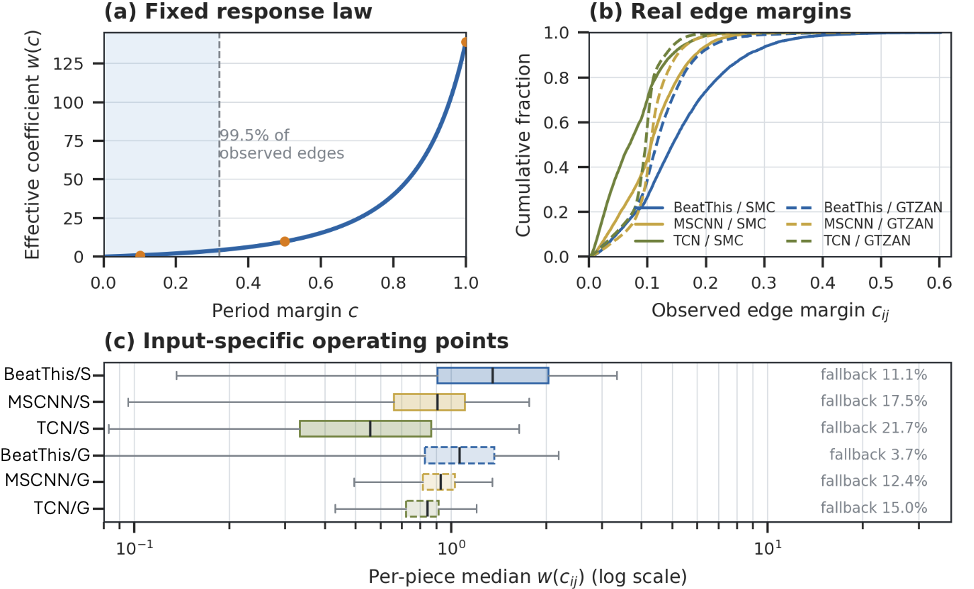
\includegraphics[width=\columnwidth]{figures/p1.jpg}
\caption{Input-conditioned duration stiffness under one frozen CASM
configuration. (a) The fixed constants map period margin $c$ to coefficient
$w(c)$; shading contains 99.5\% of observed structured-path edges. (b) Edge
margin distributions differ across backbones and corpora. (c) Per-piece median
coefficients therefore occupy different operating ranges; annotations give the
separate count-ratio fallback rate. Fixed parameters define one response law,
not one effective rigidity for every input.}
\label{fig:casm-response}
\end{figure}

\subsection{Decoding and safeguards}

A Viterbi-style dynamic program maximizes Eq.~\eqref{eq:casm-objective}, with a
restart option for an unfavourable prefix, and backtracks the highest-scoring
path. In parallel, we form the Direct path of \cite{foscarin2024beat} by
seven-frame max pooling, a zero-logit threshold, and one-frame deduplication.
If the structured-to-Direct event-count ratio falls outside
$[r_{\min},r_{\max}]$, CASM returns Direct. This is a deterministic sanity
check, not a learned router.

Downbeats are decoded only on the selected beat grid. A second dynamic program
links candidate downbeats separated by an allowed bar length and penalizes
unnecessary meter changes. Direct downbeat maxima are independently snapped to
the same beat grid; the meter path is retained only when it agrees sufficiently
with that snapped path, otherwise the snapped path is returned. Thus every
output downbeat remains synchronized with an output beat.

All scalar settings are calibrated once on development folds and then frozen
for every track and backbone, as detailed in Sec.~\ref{sec:exp}. CASM is
therefore input-conditioned but not parameter-free: it has no learned weights,
per-track tuning, annotated beats, BPM, or meter input at inference.



\section{Experiments}
\label{sec:exp}

\subsection{Evaluation protocol}
\textbf{Datasets and splits.} Following previous work, we use the publicly released data from BeatThis \cite{foscarin2024beat}, which contains 4,556 tracks from 18 beat-tracking datasets, including SMC, Hainsworth, Ballroom, Beatles, and others. This data collection provides preprocessed log-Mel spectrograms computed from 22.05kHz mono audio at 50 fps, together with a fixed eight-fold partition to conduct cross-validation experiments. For each fold, the corresponding backbone checkpoint is trained on the remaining seven folds, ensuring that evaluated tracks remain unseen during training. Among these datasets, SMC provides beat but not downbeat annotations, and is widely recognized as the hard one compared to the others. Additionally, GTZAN provides 993 tracks as the held-out evaluation set, which is excluded from the cross-validation pool.

\textbf{Backbones.} We select three models whose implementations are publicly available and readily reproducible. For BeatThis, we use the original code and pretrained checkpoints \cite{foscarin2024beat}. MSCNN is adapted from the multi-scale, multi-task convolutional network of \cite{he2026dynest}, which was designed for 60s Bark-scale specific-loudness features. We modify it to accept the 30s the unified log-Mel input and remove the task heads unrelated to beat and downbeat tracking. TCN was introduced by \cite{bock2020deconstruct}, and we use the re-implementation distributed with \cite{he2026dynest}, which has been adapted from its original 5\,s input to the same 30\,s log-Mel input, with the tempo task head removed. All resulting backbones are trained on the same data and frozen before decoding performance comparison, ensuring that every post-processor receives exactly the same 50\,Hz framewise beat/downbeat activations from a given backbone.

\textbf{Evaluation.} The eight fold-specific checkpoints of each backbone are evaluated on GTZAN and their corresponding out-of-fold SMC partitions, with scores macro-averaged over total evaluation. Following standard practice, the first 5\,s are ignored and \texttt{mir\_eval} computes F1 with a $\pm70$\,ms tolerance, CMLt, and AMLt \cite{raffel2014mireval}. CMLt measures continuity at the correct metrical level, whereas AMLt additionally accepts standard off-beat and half- or double-level interpretations.

\subsection{Post-processors and tempo support}
We compare CASM with the direct decoding, along with other post-processing methods including DBN, PLPDP \cite{chiu2023localperiodicity}, CombFilter \cite{bock2015combfilter}, and CRF beat detection \cite{korzeniowski2014crf}. Direct is the peak-picking path defined in Sec.~\ref{sec:method}, and CASM uses its fixed 30--300-BPM support. PLPDP, CombFilter, and CRF are run with their released/default parameters. For methods without a joint beat/downbeat decoder, downbeats are decoded from the downbeat activation stream and snapped to the corresponding beat grid.

DBN receives separate treatment because its behaviour is particularly sensitive to global tempo support. We use the standard joint \texttt{madmom} configuration \cite{krebs2015dbn}: meters $\{3,4\}$, transition weight 100, observation weight 16, threshold 0.05, and the default 55--215-BPM range. Since many SMC data are fall below 55 BPM \cite{ahn2026smcblindspot}, Table~\ref{tab:postprocessor_ablation} also explores a 30--300-BPM DBN variant in which only the tempo range is changed. For a matched diagnostic, we additionally report CASM with its support restricted to 55--215 BPM on BeatThis activations, with all other CASM settings remain unchanged.

\subsection{CASM calibration}
CASM has no learned weights or random seed. The final configuration used in all main tables is calibrated once on the union of SMC folds 1--7 (7F) and then frozen for every track, backbone, and dataset. The same global scalar settings are therefore used on BeatThis, MSCNN, and TCN, on both SMC and GTZAN, without per-track or per-dataset BPM, meter, or parameter tuning at inference. Because the aggregate SMC results use eight-fold out-of-fold backbone activations while the decoder configuration is calibrated on folds 1--7, they are out-of-fold with respect to backbone training but are not a nested estimate of decoder calibration.

We analyse calibration-data sensitivity separately rather than using it to choose the main operating point. SMC fold 0 is held out from decoder calibration throughout. From folds 1--7, we enumerate every 1-, 2-, and 4-fold calibration subset ($7$, $21$, and $35$ combinations) and the seven-fold union. For both CASM and DBN, a decoder configuration is selected independently on each calibration subset and then evaluated on the same fixed SMC-fold-0 panel and on GTZAN using one fixed backbone seed. The resulting distributions therefore measure sensitivity to the amount and composition of calibration data, while the 7F CASM configuration is the maximally supported global configuration used for the main results.

\section{Results}
\label{sec:results}

\subsection{Comparison with post-processors}

\begin{table}[t]
\centering
\caption{Post-processing comparison on fixed backbone activations. Direct rows report absolute scores; post-processor rows report changes from Direct. DBN default uses 55--215 BPM, while wide-support variants use 30--300 BPM to cover low-tempo SMC tracks \cite{ahn2026smcblindspot}, all other settings are unchanged.}
\label{tab:postprocessor_ablation}
\begingroup
\fontsize{7.5pt}{8.5pt}\selectfont
\setlength{\tabcolsep}{0.7pt}
\renewcommand{\arraystretch}{0.92}
\resizebox{\columnwidth}{!}{%
\begin{tabular}{l|c|rrr@{\hspace{2pt}}|rrr@{\hspace{2pt}}|rrr}
\toprule
\multicolumn{1}{c|}{\multirow{2}{*}{\textbf{Method}}}
& \multicolumn{1}{c|}{\multirow{2}{*}{\textbf{BPM}}}
& \multicolumn{6}{c|}{\textbf{GTZAN (Beat / Downbeat)}}
& \multicolumn{3}{c}{\textbf{SMC (Beat)}} \\
\cmidrule(lr){3-8}
\cmidrule(l){9-11}
& & F1 & CMLt & AMLt
& F1 & CMLt & AMLt
& F1 & CMLt & AMLt \\
\midrule

\textbf{BeatThis} (direct) \cite{foscarin2024beat}
& --
& 89.1 & 79.8 & 89.8
& 78.3 & 67.2 & 79.1
& 62.7 & 51.4 & 61.0 \\

w. CASM
& 30-300
& \heatposbest{0.3} & \heatposbest{0.8} & \heatpos{1.2}
& \heatposbest{0.7} & \heatpos{3.6} & \heatpos{8.0}
& \heatposbest{0.3} & \heatposbest{2.4} & \heatposbest{3.6} \\

w. CASM, ablation
& 55-215
& \heatpos{0.1} & \heatpos{0.5} & \heatpos{0.6}
& \heatpos{0.5} & \heatpos{2.9} & \heatpos{5.8}
& \heatpos{0.1} & \heatpos{0.4} & \heatpos{2.0} \\

w. DBN \cite{krebs2015dbn}
& 30-300
& \heatneg{0.5} & \heatneg{0.9} & \heatpos{0.2}
& \heatneg{1.5} & \heatneg{0.6} & \heatpos{1.1}
& \heatneg{1.6} & \heatpos{0.4} & \heatpos{3.5} \\

w. DBN, default
& 55-215
& \heatneg{1.0} & \heatpos{0.7} & \heatpos{1.3}
& \heatneg{0.9} & \heatposbest{6.2} & \heatposbest{8.7}
& \heatneg{5.2} & \heatneg{3.9} & \heatpos{1.5} \\

% w. PLPDP
% & 55--215
% & \heatneg{0.1} & \heatposbest{0.8} & \heatpos{0.1}
% & \heatneg{0.2} & \heatpos{0.1} & \heatneg{0.1}
% & \heatneg{1.4} & \heatneg{4.7} & \heatpos{0.5} \\

w. PLPDP \cite{chiu2023localperiodicity}
& 30-300
& \heatpos{0.1} & \heatpos{0.3} & \heatpos{0.3}
& \heatpos{0.1} & \heatpos{0.2} & \heatpos{0.2}
& \heatneg{0.9} & \heatneg{3.5} & \heatneg{0.3} \\

w. CombFilter \cite{bock2015combfilter}
& 30-300
& \heatneg{4.0} & \heatneg{3.6} & \heatpos{0.1}
& \heatneg{3.3} & \heatpos{3.2} & \heatpos{7.6}
& \heatneg{7.1} & \heatpos{1.1} & \heatpos{3.1} \\

w. CRF \cite{korzeniowski2014crf}
& 30-300
& \heatneg{0.6} & \heatneg{0.3} & \heatposbest{1.4}
& \heatneg{1.4} & \heatpos{1.9} & \heatpos{5.5}
& \heatneg{1.2} & \heatpos{1.4} & \heatpos{1.2} \\

\midrule
\textbf{MSCNN} (direct) \cite{he2026dynest}
& --
& 86.1 & 73.4 & 79.9
& 70.8 & 53.1 & 63.1
& 57.2 & 42.0 & 48.4 \\

w. CASM
& 30--300
& \heatposbest{0.4} & \heatpos{1.6} & \heatpos{2.4}
& \heatpos{1.5} & \heatpos{12.5} & \heatpos{18.3}
& \heatposbest{0.3} & \heatposbest{3.5} & \heatposbest{6.8} \\
w. DBN
& 30--300
& \heatneg{1.1} & \heatpos{0.2} & \heatpos{5.9}
& \heatneg{0.9} & \heatpos{9.5} & \heatpos{14.6}
& \heatneg{0.2} & \heatpos{2.2} & \heatpos{4.1} \\
w. DBN, default
& 55--215
& \heatneg{0.6} & \heatposbest{4.0} & \heatposbest{7.2}
& \heatposbest{1.8} & \heatposbest{15.8} & \heatposbest{21.2}
& \heatneg{4.9} & \heatpos{0.3} & \heatpos{3.9} \\
\midrule

\textbf{TCN} (direct) \cite{bock2020deconstruct}
& --
& 87.1 & 73.8 & 81.7
& 62.4 & 24.6 & 59.9
& 52.9 & 30.1 & 36.0 \\
w. CASM
& 30--300
& \heatposbest{0.3} & \heatposbest{1.3} & \heatpos{1.6}
& \heatpos{2.1} & \heatpos{9.2} & \heatpos{13.4}
& \heatposbest{1.7} & \heatposbest{4.5} & \heatposbest{8.2} \\
w. DBN
& 30--300
& \heatneg{1.9} & \heatneg{0.8} & \heatpos{4.4}
& \heatneg{0.2} & \heatpos{8.9} & \heatpos{9.3}
& \heatneg{0.4} & \heatpos{2.1} & \heatpos{5.9} \\
w. DBN, default
& 55--215
& \heatneg{2.6} & \heatneg{0.7} & \heatposbest{5.0}
& \heatposbest{4.9} & \heatposbest{23.2} & \heatposbest{22.9}
& \heatneg{0.9} & \heatneg{7.0} & \heatpos{2.3} \\
% w. CombFilter
% & --
% & \heatneg{6.3} & \heatpos{1.1} & \heatpos{4.3}
% & \heatneg{2.2} & \heatpos{12.2} & \heatpos{19.5}
% & \heatneg{5.7} & \heatpos{9.3} & \heatpos{17.9} \\
% w. CRF
% & --
% & \heatpos{0.7} & \heatpos{3.3} & \heatpos{7.8}
% & \heatpos{1.5} & \heatpos{4.8} & \heatpos{18.3}
% & \heatneg{2.3} & \heatneg{2.2} & \heatpos{12.4} \\

\bottomrule
\end{tabular}%
}
\endgroup
\end{table}

Table~\ref{tab:postprocessor_ablation} isolates the post-processor by holding the backbone activations fixed. With 30--300-BPM support, the CASM improves BeatThis (direct pick-peaking) on every reported F1, CMLt, and AMLt entry across all three backbones and both datasets. Relative to DBN, CASM generally preserves F1 better, while DBN can produce larger continuity gains, particularly for GTZAN downbeats. The large SMC change between the 55--215- and 30--300-BPM DBN variants also shows how strongly a fixed DBN can depend on its global tempo range. PLPDP, CombFilter, and CRF provide useful alternatives, but none improves every reported metric under the same fixed activations. Overall, CASM gives a conservative F1--continuity operating point that transfers across backbone families without changing decoder parameters.

\subsection{Comparison with the state of the art}

\begin{table}[t]
\centering
\caption{Comparison with recent beat-tracking systems. BeatThis (direct) and CASM results were obtained from our experiments, while all other values are reported from their original papers.}
\label{tab:audiodyn_cross_dataset_sota}
\begingroup
\fontsize{8pt}{11pt}\selectfont
\setlength{\tabcolsep}{0.5pt}
\renewcommand{\arraystretch}{1.0}
\resizebox{\columnwidth}{!}{%
\begin{tabular}{l|ccc|ccc|ccc}
\toprule
\multicolumn{1}{c|}{\multirow{2}{*}{\textbf{Method}}}
& \multicolumn{6}{c|}{\textbf{GTZAN (Beat / Downbeat)}}
& \multicolumn{3}{c}{\textbf{SMC (Beat)}} \\
\cmidrule(lr){2-4}
\cmidrule(lr){5-7}
\cmidrule(l){8-10}
& F1 & CMLt & AMLt
& F1 & CMLt & AMLt
& F1 & CMLt & AMLt \\
\midrule
\rowcolor{gray!10}
\textbf{HN-MERT} w. DBN \cite{ru2025hingenet}
& \textbf{89.7} & 81.4 & \textbf{94.3}
& 77.4 & 71.6 & 87.2
& 61.7 & -- & -- \\
\textbf{HN-MusicFM} w. DBN
& 89.2 & 80.9 & 93.7
& \textbf{79.8} & 73.2 & \textbf{89.5}
& 60.6 & -- & -- \\
\rowcolor{gray!10}
\textbf{BeatFM-MERT} w. DBN \cite{ru2025beatfm}
& \underline{89.5} & \underline{82.7} & \underline{93.9}
& 76.7 & 70.2 & 85.4
& 61.3 & -- & -- \\
\textbf{BeatFM-MusicFM} w. DBN
& 89.1 & 80.6 & 93.5
& \underline{79.6} & \underline{74.4} & \underline{88.7}
& 60.5 & -- & -- \\
% \textbf{SpecTNT-TCN} w. DBN \cite{hung2022modeling}
% & 88.7 & 81.2 & 92.0
% & 75.6 & 71.5 & 88.1
% & 60.5 & 51.4 & 66.3 \\
% \textbf{TCN} + DBN  \cite{bock2020deconstruct}
% & 88.5 & 81.3 & 93.1
% & 67.2 & 64.0 & 83.2
% & 55.2 & 46.5 & 64.3 \\
\rowcolor{gray!10}
\textbf{BeatMamba} w. DBN \cite{ru2026beatmamba}
& 88.9 & 82.3 & \textbf{94.3}
& -- & -- & --
& 58.7 & 46.8 & 62.4 \\
\textbf{BeatKAN} w. DBN \cite{zhang2025beatkan}
& 88.2 & 78.1 & 92.3
& -- & -- & --
& 59.8 & 48.4 & 64.0 \\
\rowcolor{gray!10}
\textbf{MDM-BeatThis} (direct) \cite{foscarin2026masked}
& \textbf{89.7} & \textbf{82.9} & 92.5
& 79.5 & \textbf{76.4} & 88.5
& 61.0 & 48.9 & \underline{64.3} \\
\midrule
\textbf{BeatThis} (direct) \cite{foscarin2024beat}
& 89.1 & 79.8 & 89.8
& 78.3 & 67.2 & 79.1
& \underline{62.7} & \underline{51.4} & 61.0 \\
% \textbf{BeatThis} w. DBN (default \& opt)
% & 88.1 & 80.5 & 91.1
% & 77.4 & 73.4 & 87.8
% & 57.5 & 47.5 & 62.5 \\
\rowcolor{gray!10}
\textbf{BeatThis} w. CASM
& 89.4 & 80.6 & 91.0
& 79.0 & 70.8 & 87.1
& \textbf{63.0} & \textbf{53.8} & \textbf{64.6} \\
\bottomrule
\end{tabular}%
}
\endgroup
\end{table}

Table~\ref{tab:audiodyn_cross_dataset_sota} compares the BeatThis works with CASM results with recent literature. While using CASM improves six beat/downbeat metrics compared to BeatThis (directly peak-picking) on the GTZAN, we reported the highest scores on SMC compared to the other SOTA systems. On GTZAN, stronger task-specific or pre-trained frontends retain the best individual scores. The literature table therefore provides system-level context; controlled claims about decoder behaviour come from Table~\ref{tab:postprocessor_ablation}, where the backbone activations are held fixed.

\subsection{Sensitivity to calibration data}
The sensitivity experiment keeps the evaluation panels fixed and changes only the data used to calibrate the decoder. For each calibration scale $k\in\{1,2,4,7\}$, CASM and DBN are calibrated on the corresponding SMC fold subsets described in Sec.~\ref{sec:exp}, and every selected configuration is evaluated on the same held-out SMC fold 0 and the same GTZAN backbone seed. Thus, the spread at a given scale measures dependence on which calibration folds were used, while the movement of the distribution centre measures how additional calibration data changes transfer to the two fixed evaluation panels.

\begin{figure}[h]
\begin{center}
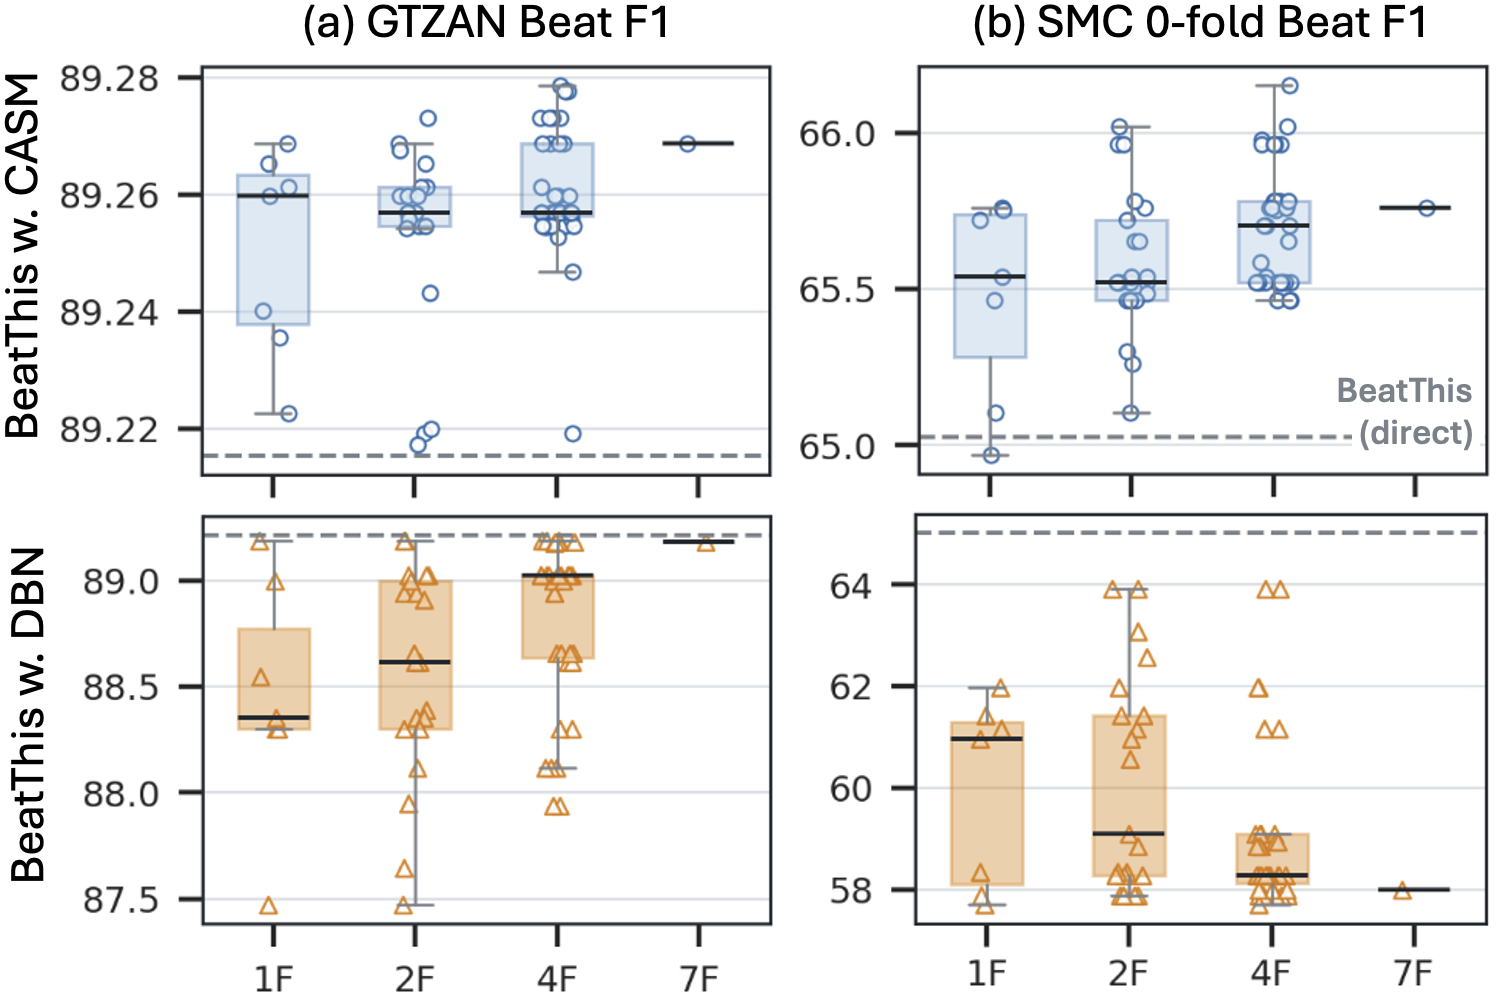
\includegraphics[width=0.9\columnwidth]{figures/p2.jpg}
\caption{Sensitivity to calibration data for CASM and DBN. Each point corresponds to a decoder configuration selected from one of the $7/21/35$ exhaustive 1-/2-/4-fold subsets of SMC folds 1--7 and evaluated on fixed SMC-fold-0 and GTZAN panels; 7F is a single configuration. Boxes are descriptive because calibration subsets overlap, and dashed lines show Direct performance.}
\label{fig:calibration-scale}
\end{center}
\end{figure}

Fig.~\ref{fig:calibration-scale} shows a clear difference in calibration behaviour. CASM remains tightly clustered across fold combinations, and its central performance improves consistently as more calibration folds are used on both the held-out SMC panel and GTZAN. In contrast, DBN exhibits much wider variation across calibration subsets, and the trends on SMC and GTZAN do not move together: configurations favoured by one panel can transfer poorly to the other. This cross-dataset disagreement is consistent with stronger calibration-set over-specialisation in the fixed DBN parameterisation. The 7F CASM setting used in the main tables is therefore supported by the full available calibration pool rather than selected from a favourable smaller-fold combination.

\section{Conclusion and Future Work}
\label{sec:concl}

CASM revisits structured beat decoding as an inductive bias conditioned on each input, not as a return to a fixed global grid. It joins activation-supported events with locally centred segment potentials and deliberately relaxes those potentials when periodic evidence is ambiguous. Once globally calibrated, the same deterministic module runs without upstream retraining, user annotation, or per-track tempo and meter settings. Current evidence supports a conservative F1--continuity alternative to Direct and DBN decoding, not universal dominance. The next version should use strict nested or leave-one-dataset-out calibration, matched tempo-support baselines, PLPDP and mechanism ablations, and explicit safeguard statistics. Multi-hypothesis period paths, causal decoding, and a differentiable duration layer are natural extensions, as is evaluation on every recent tracker that releases compatible activations.

\bibliographystyle{IEEEbib}
\bibliography{casm}

\end{document}